\documentclass{article}
\usepackage[utf8]{inputenc}
\usepackage[T1]{fontenc}
\usepackage{graphicx}
\begin{document}
\title{Referat af vejledermøde}
\author{SW2-A405a}
\date{24. marts 2014}
\maketitle
\section{Problemformulering}
Brian godkender problemformuleringen.

\section{Use cases / user stories - Hvordan gøres dette bedst?}
Usecases kan tegnes nemt grafisk. På den ene sider roller, og på den anden side funktioner. vigtige spørgsmpl vilke forspørgelser, stilles der til systemet?

User stories: agil udvikling. Bruger skriver selv en forklaring af hvordan han gerne vil bruge systemet.

Simon: er det havnefogeden? Brian: det er lidt svært med jeres, men normalt er det slutbrugeren.

En tredje måde er sekvens diagrammer. Det er målrettet imod at demonstrere komplekse interaktionssenarier. Eksempel; Roller har tidslinjer, hvor der sætters forbindelse imellem forskellige rollers tidslinjer, på punkter hvor der er interaktion.

\begin{figure}[h]
  \caption{Brians eksempel på et sekvens diagram}
  \centering
    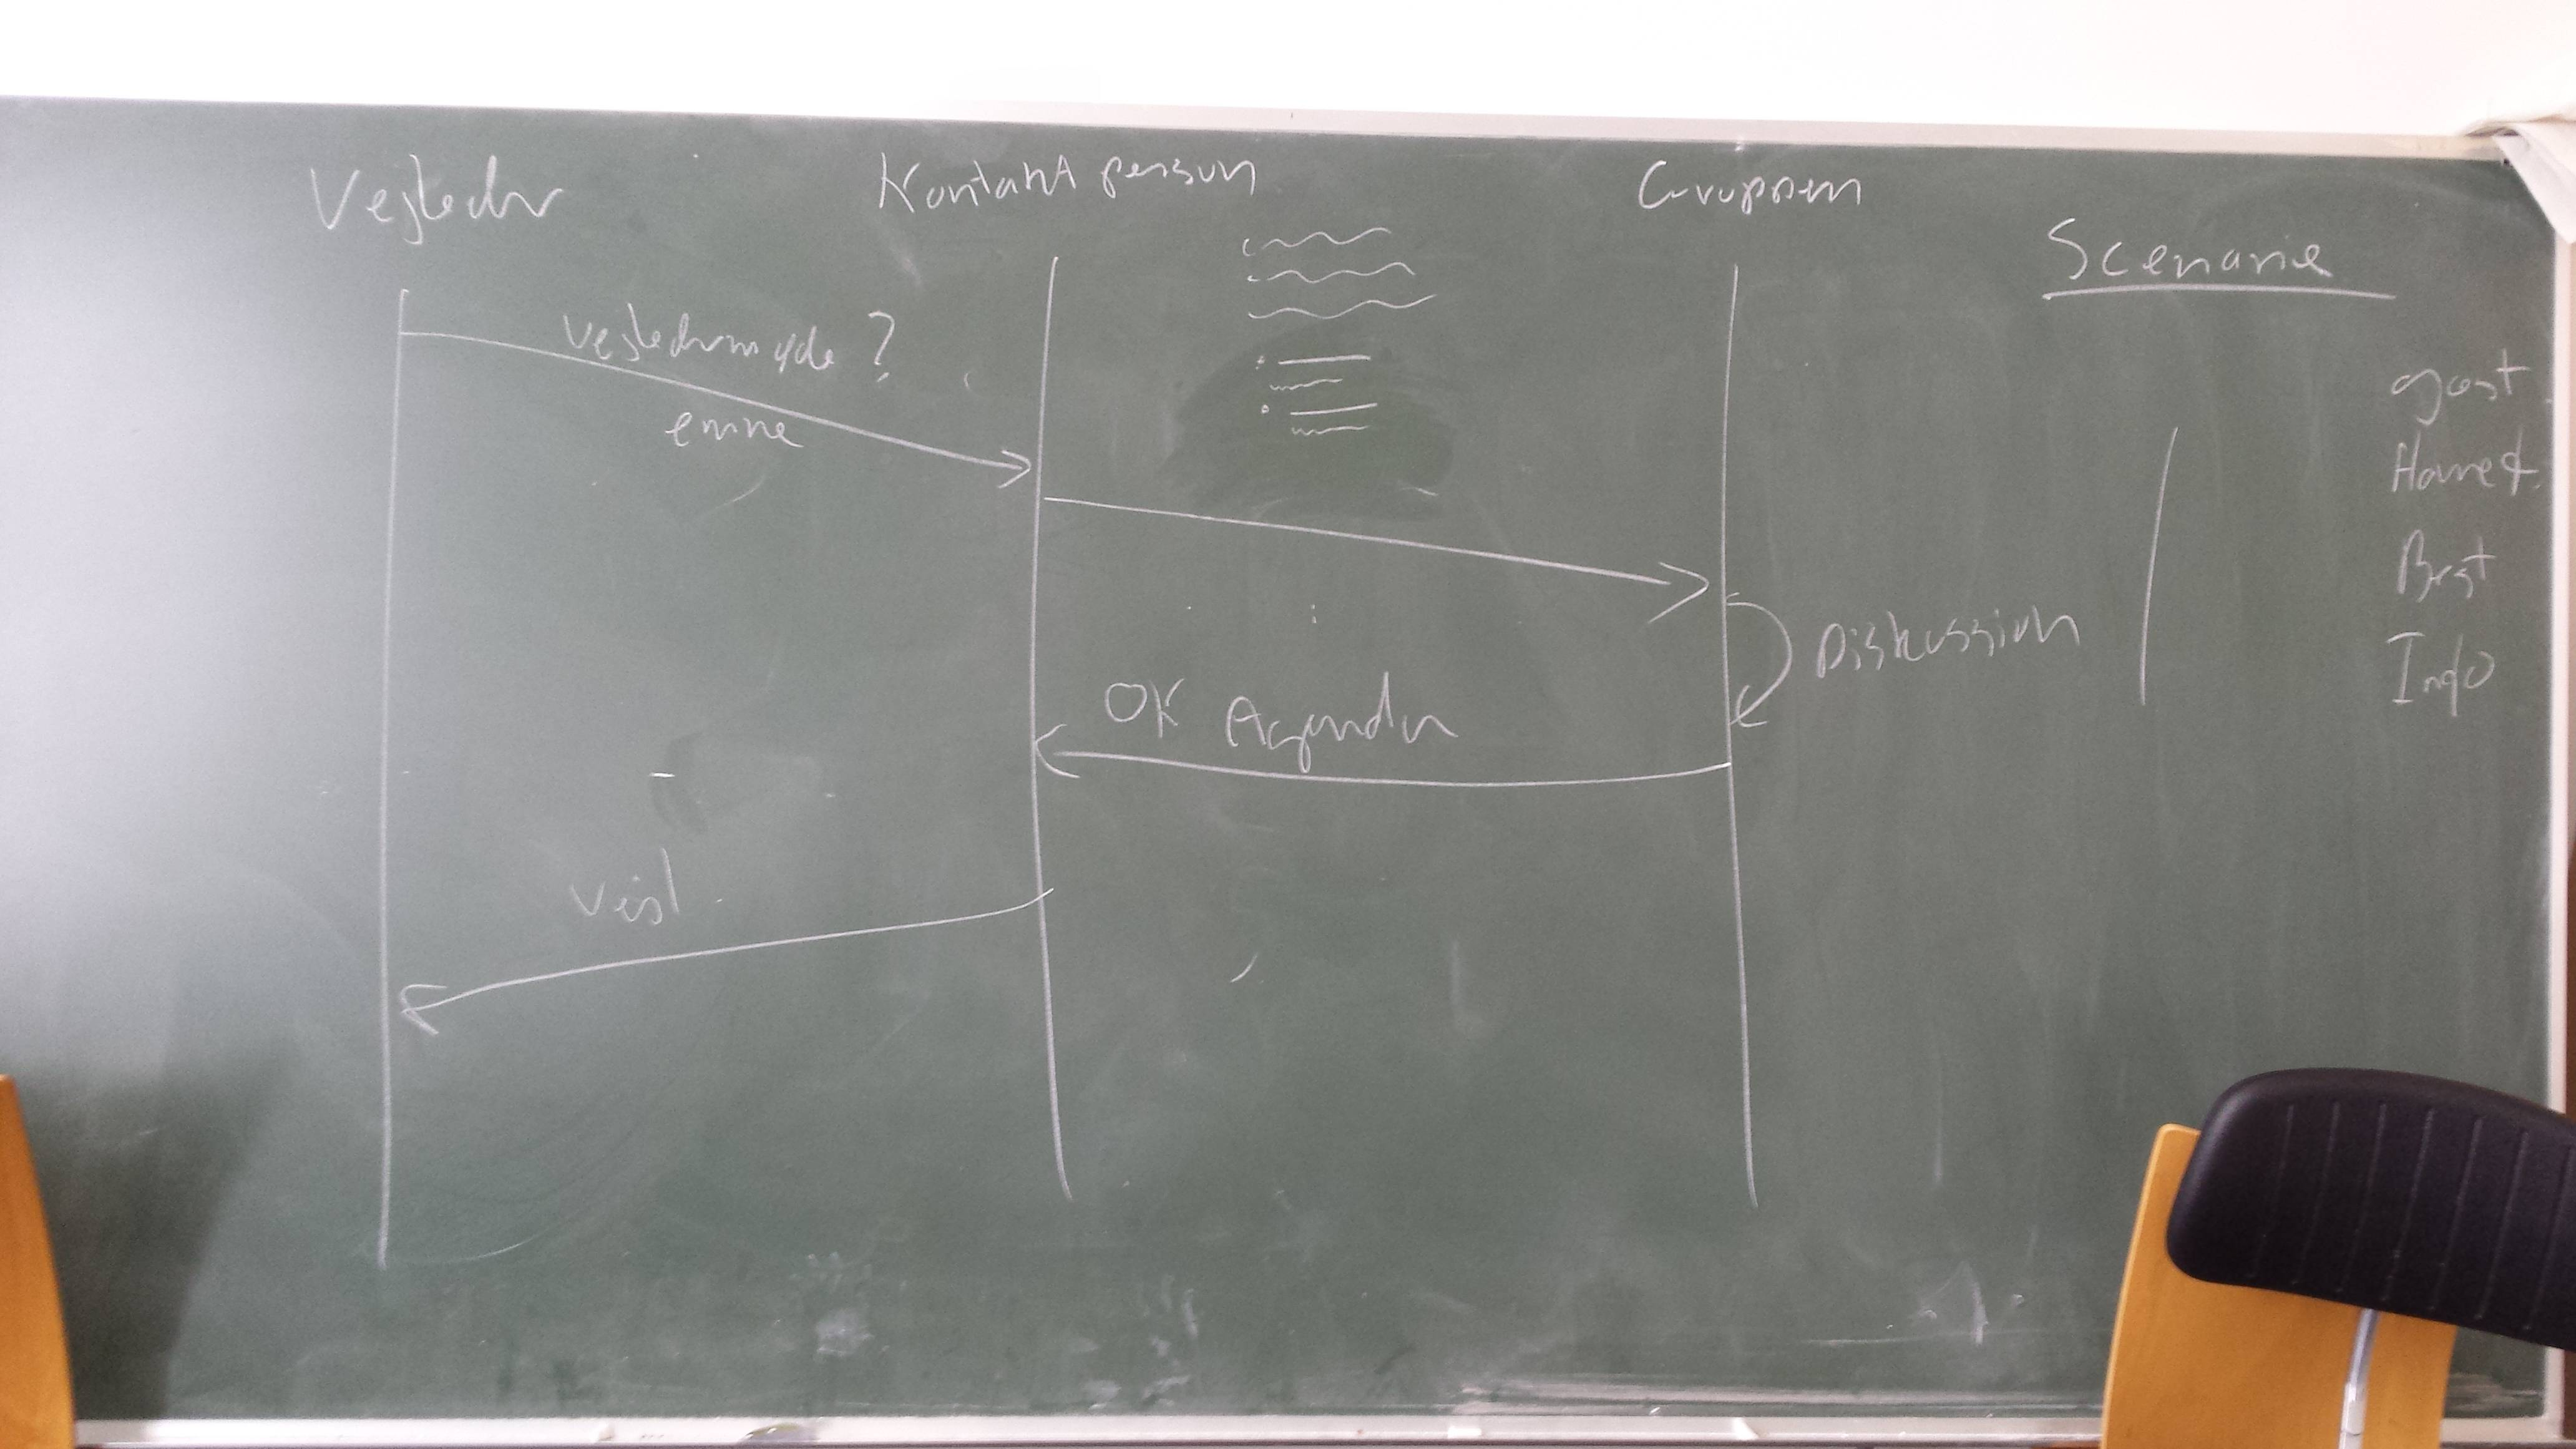
\includegraphics[width=1\textwidth]{sekvensdiagrammer}
\end{figure}

Brian foreslår brug af usecases, og ikke user stories, da de er mindre rigide.

Brug usecases som et redskab sålænge at det er væsentligt.

\section{Er teknologien realistisk (sensor og aktuator). Hvordan gør vi det?}

Simon: emulerer vi bare vores sensorer?

Brian: Ja.

Alexander: Hvor realistisk er bådgenkendelse.

Brian: det er ikke urealistisk at både kan være tagget (enten RFID el. lign.). Det er heller ikke urealistisk at både om 10 års tid har computere som kan sende denne slags data. 

Lav 1-2 sider omkring hvad vi tænker mht. teknologi vi gerne ser eksisterende. Hvilke krav vi har til hardware (sensorer \& lamper). Lidt omkring tags på bådene. Aktiv RFID eksistere allerede. 

\section{GUI vs CLI}

Simon: vi vil gerne først lave gui når vi HAR lavet det andet.

Brian: rigtig måde at gøre det på. Man kan om end lave et skærmbillede af hvad man vil have. Implementation kan komme senere.

Mht. til valg af GUI typer: drag'n'drop kan være godt til prototyper, men de brede platforme er mere professionelle.

\section{Test driven development - tilgang til programmering}

Relativt konkret niveau. Skriv testcase for funktioner først. Hvad er ønsket input og hvad er ønsket output. Skriv små dele først. Test, og så skriv mere på hvis der ikke var fejl.

Testframework: visual studio har unit-test indbygget. Hvis i alle skriver i visual studio, så brug det.

Test-case er en specifikation for funktioner.

Brian: hvor ser jeres tidsplan ud.

Gruppen: vi har ikke fastsat noget.

Brian: overvej at kvantifisere tiden til.

Mht. database vs. fil, siger brian: gør det der er nemmest. Pas på med at gøre mere arbejde end hvad der gives af udbytte. Begge dele er fint med vejleder, bare det er god datahåndtering.
\end{document}